% $Id: appendix.tex 124799 2018-11-23 12:14:45Z pkoppenb $
% ===============================================================================
% Purpose: appendix to the standard template: standard symbol alises from Ulrik
% Author: Tomasz Skwarnicki
% Created on: 2009-09-24
% ===============================================================================

%{\noindent\normalfont\bfseries\Large Appendices}
% \section*{Appendices}

\appendix

% \input{supplementary-app}


\clearpage
\renewcommand{\thefigure}{S\arabic{figure}}
\renewcommand{\thetable}{S\arabic{table}}
\renewcommand{\theequation}{S\arabic{equation}}

\setcounter{equation}{0}
\setcounter{figure}{0}
\setcounter{table}{0}
\setcounter{page}{1}

{\noindent\normalfont\bfseries\Large Supplementary Material}\\

%\begin{figure}[!h]
%   \begin{center}
%      \includegraphics[width=0.48\linewidth]{figures/2DPlot_Kmm_forPaper.pdf}
%      \hfill
%      \includegraphics[width=0.48\linewidth]{figures/2DPlot_Kee_forPaper.pdf}
%   \end{center}
%   \vspace*{-0.5cm}
%   \caption{Two-dimensional distributions of $(\mKll,\qsq)$ for  (left) muon and (right) electron candidates. In the muon plot the nonresonant signal candidates can be seen as a vertical band around the \Bp mass. The diagonal bands show contributions from the \BuJpsiK and \BuPsiK decays. The horizontal bands show combinatorial backgrounds formed with the \jpsi and \psitwos resonances. In the electron plot the distribution of all of these components is smeared by the bremsstrahlung and the bremsstrahlung recovery process.}\label{fig:2Dplot}
%\end{figure}

\subsection*{Branching fraction measurements}

The comparison of the \BuKmm branching fraction from Ref.~\cite{LHCb-PAPER-2014-006} to the \BuKee branching fraction resulting from the measurement of \RK presented in this paper is shown in Fig.~\ref{fig:BFs}. The uncertainty stemming from the branching fractions of the corresponding normalisation channels is folded into the total uncertainty of each measurement.

\begin{figure}[h]
    \centering
    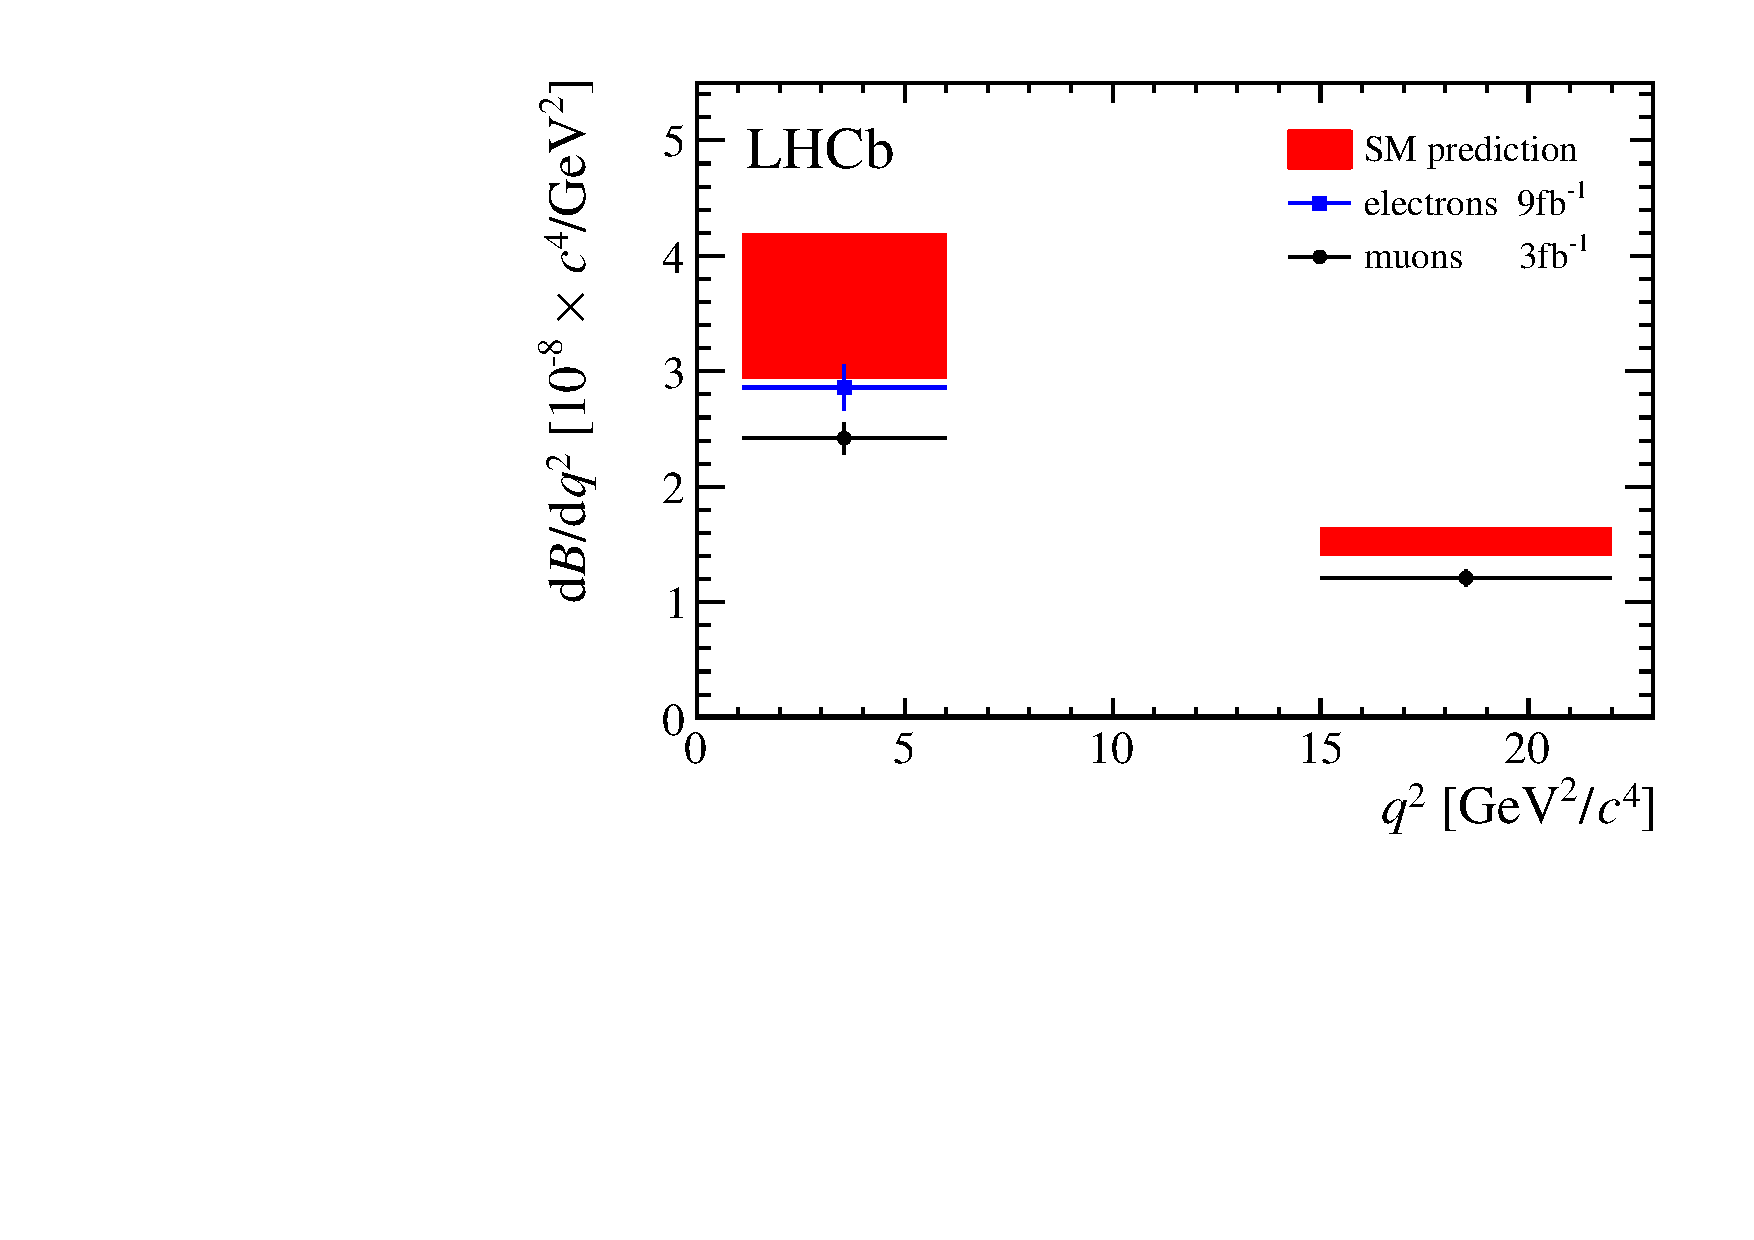
\includegraphics[width=0.7\textwidth]{figures/FigS1.pdf}
    \caption{Branching fractions of (blue) \BuKee from this paper and (black) \BuKmm from Ref.~\cite{LHCb-PAPER-2014-006} including the \qsq bin $15.0<\qsq<22.0\gevgevcccc$. The SM predictions (red area) from Refs.~\cite{Bailey:2015dka,Du:2015tda} are also shown.}
    \label{fig:BFs}
\end{figure}

\clearpage

\subsection*{Fits to the {\boldmath{\BuPsiK}} resonant mode }

The fits to the resonant \BuPsiK decay mode in different data-taking periods and trigger categories are shown in Fig.~\ref{fig:resPsi2Sfits_categories}. The strong correlation between the combinatorial background and the partially reconstructed decays from higher charmonium resonances causes the variation of the fitted mass shapes across data-taking periods and trigger categories. However, this has a negligible effect on the signal yield extraction as the sum of the two contributions is constant across data-taking periods and trigger categories.


\clearpage

\begin{figure}
    \centering
    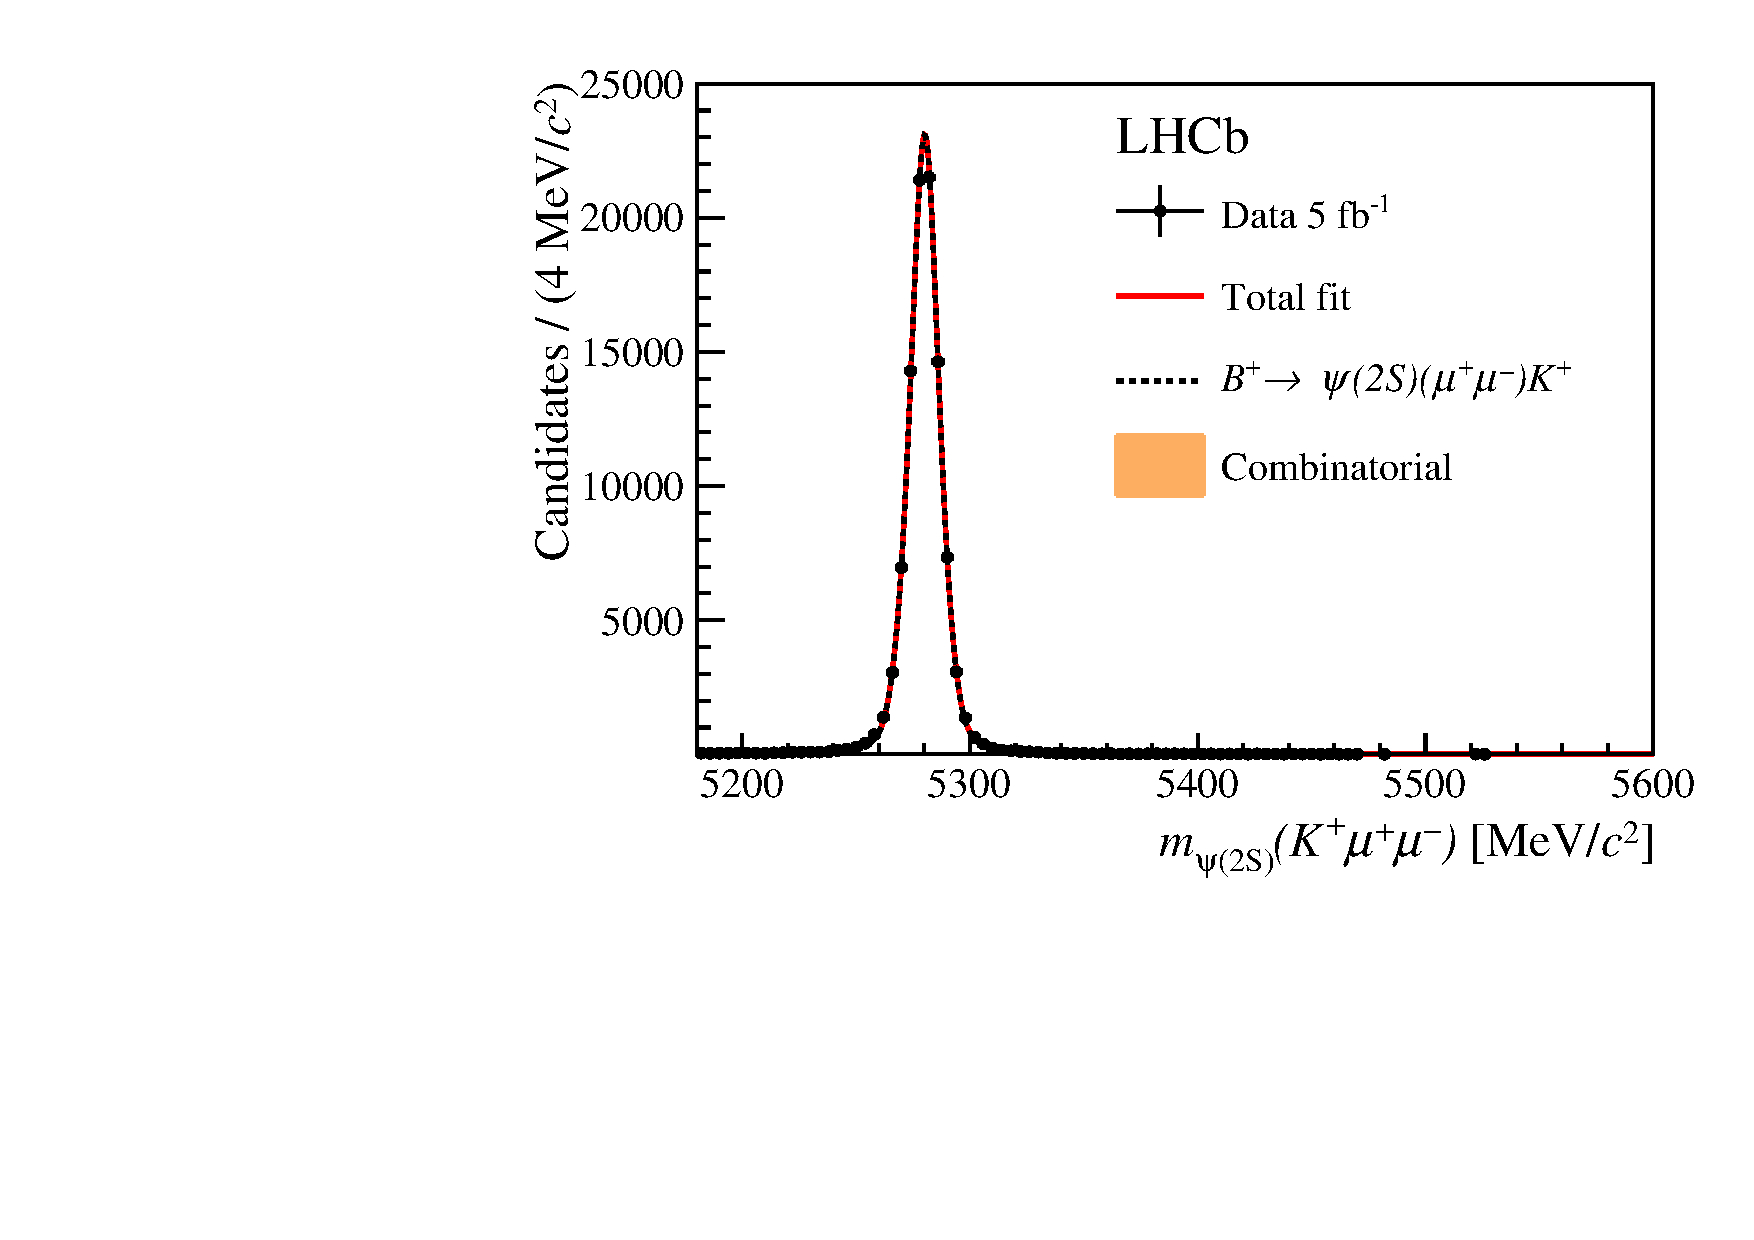
\includegraphics[width=0.45\textwidth]{figures/FigS2a.pdf}
    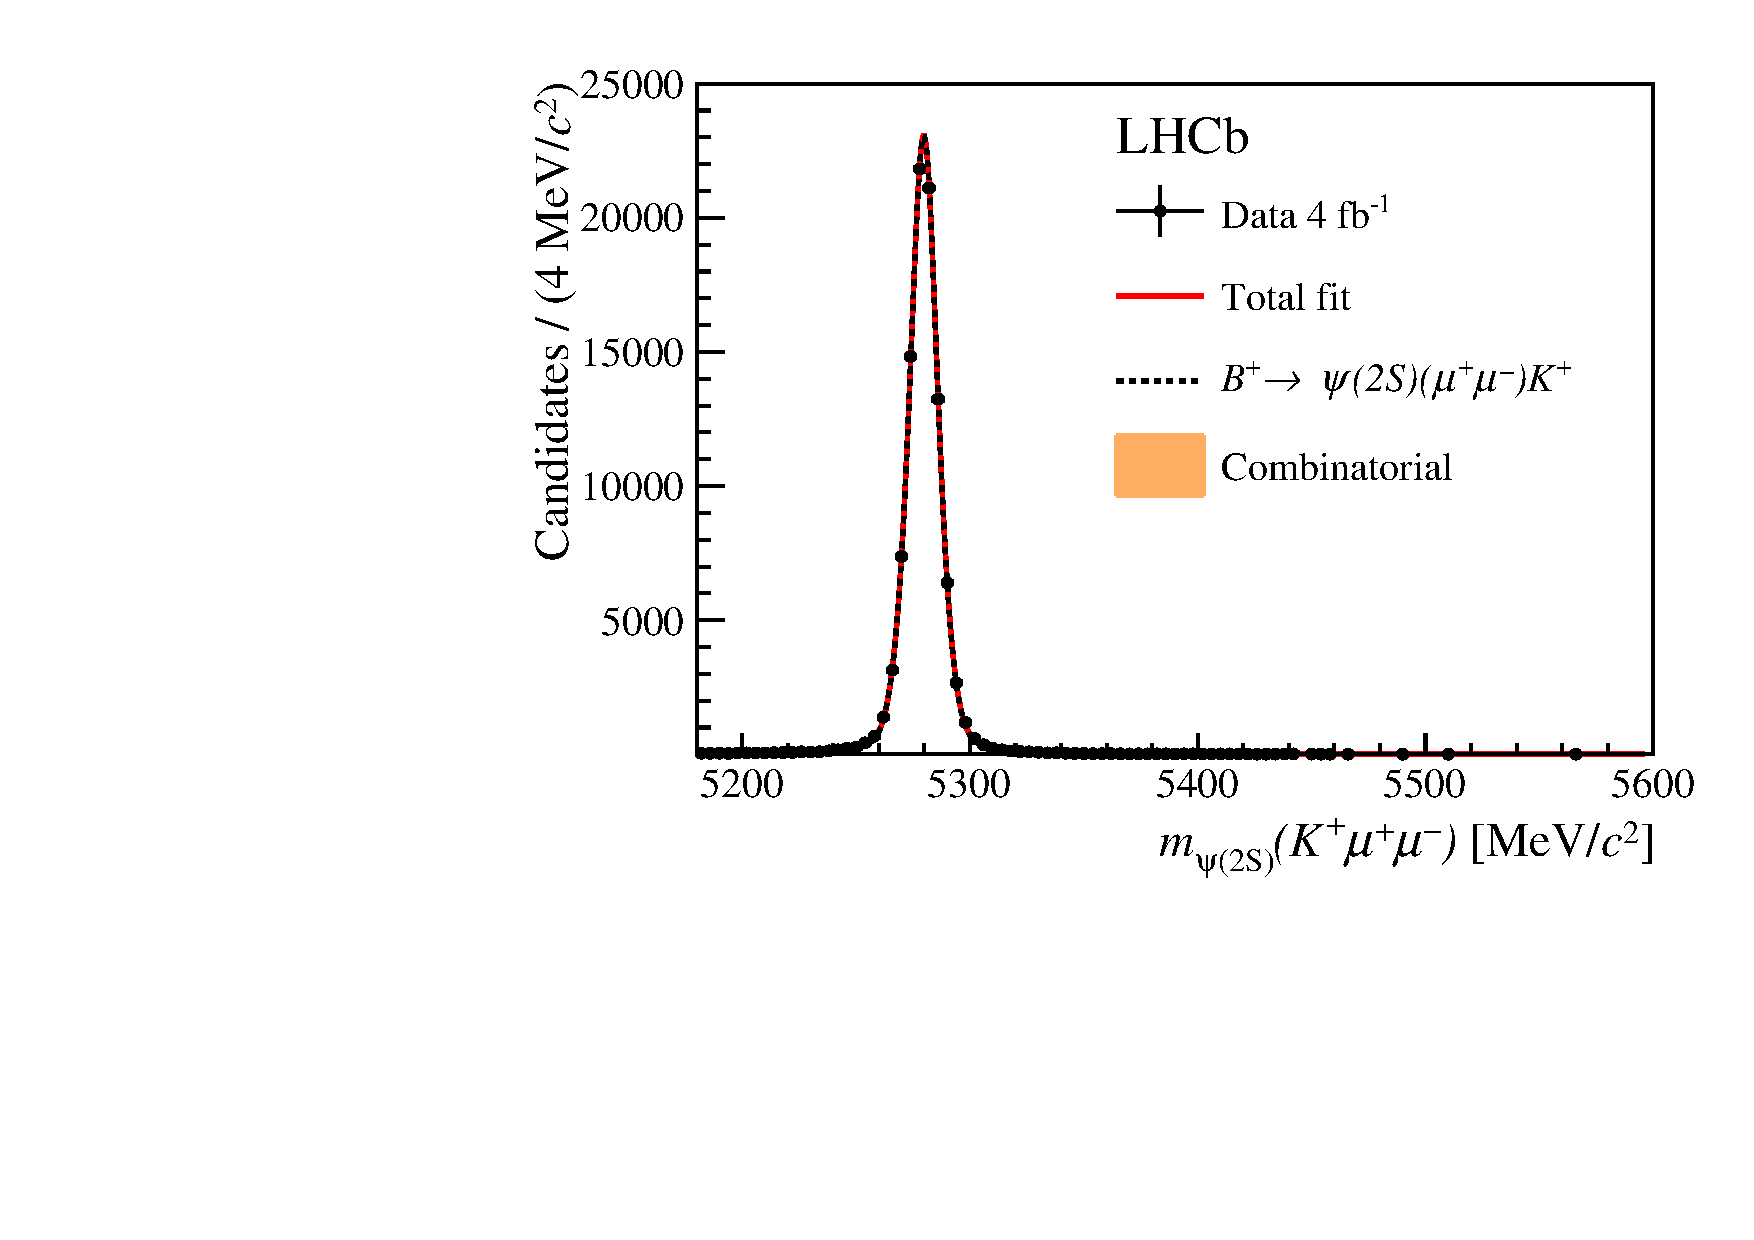
\includegraphics[width=0.45\textwidth]{figures/FigS2b.pdf}
    
    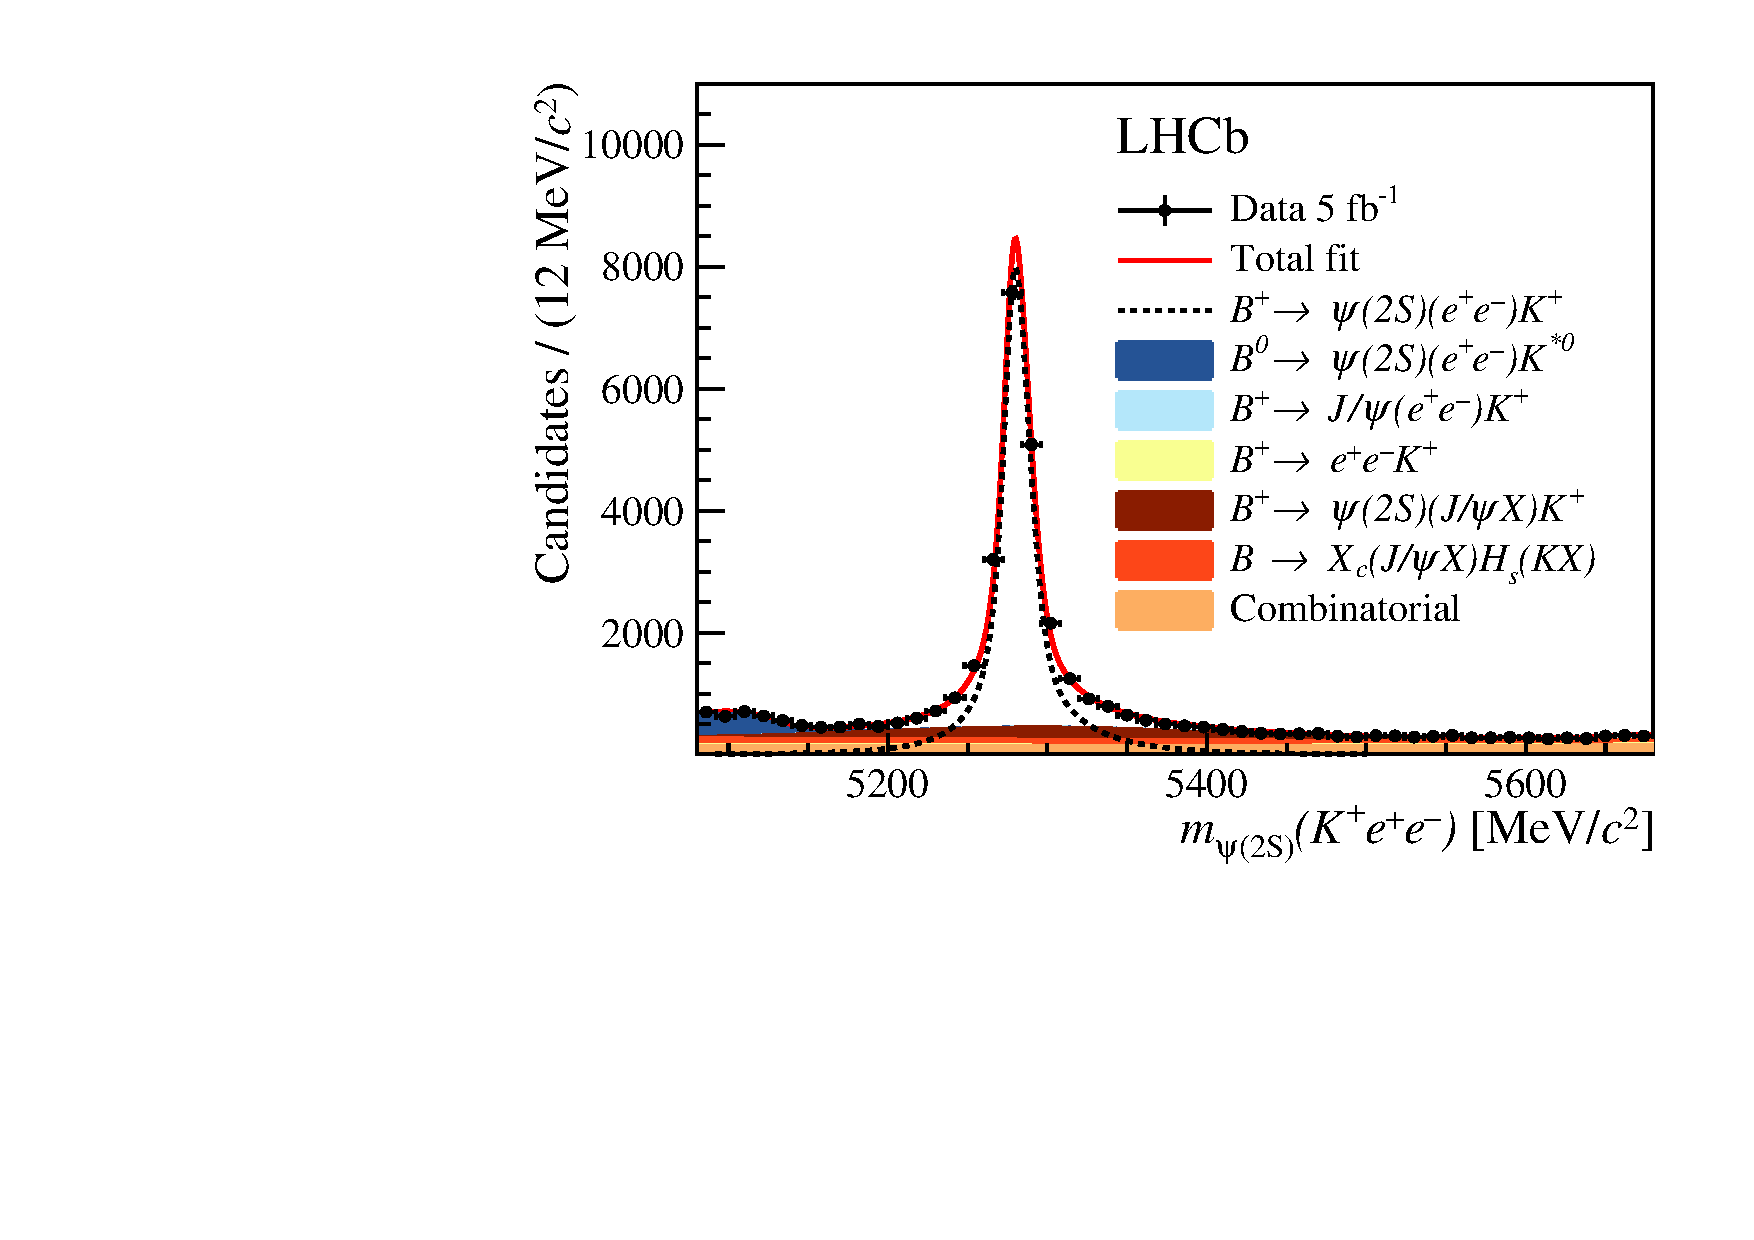
\includegraphics[width=0.45\textwidth]{figures/FigS2c.pdf}
    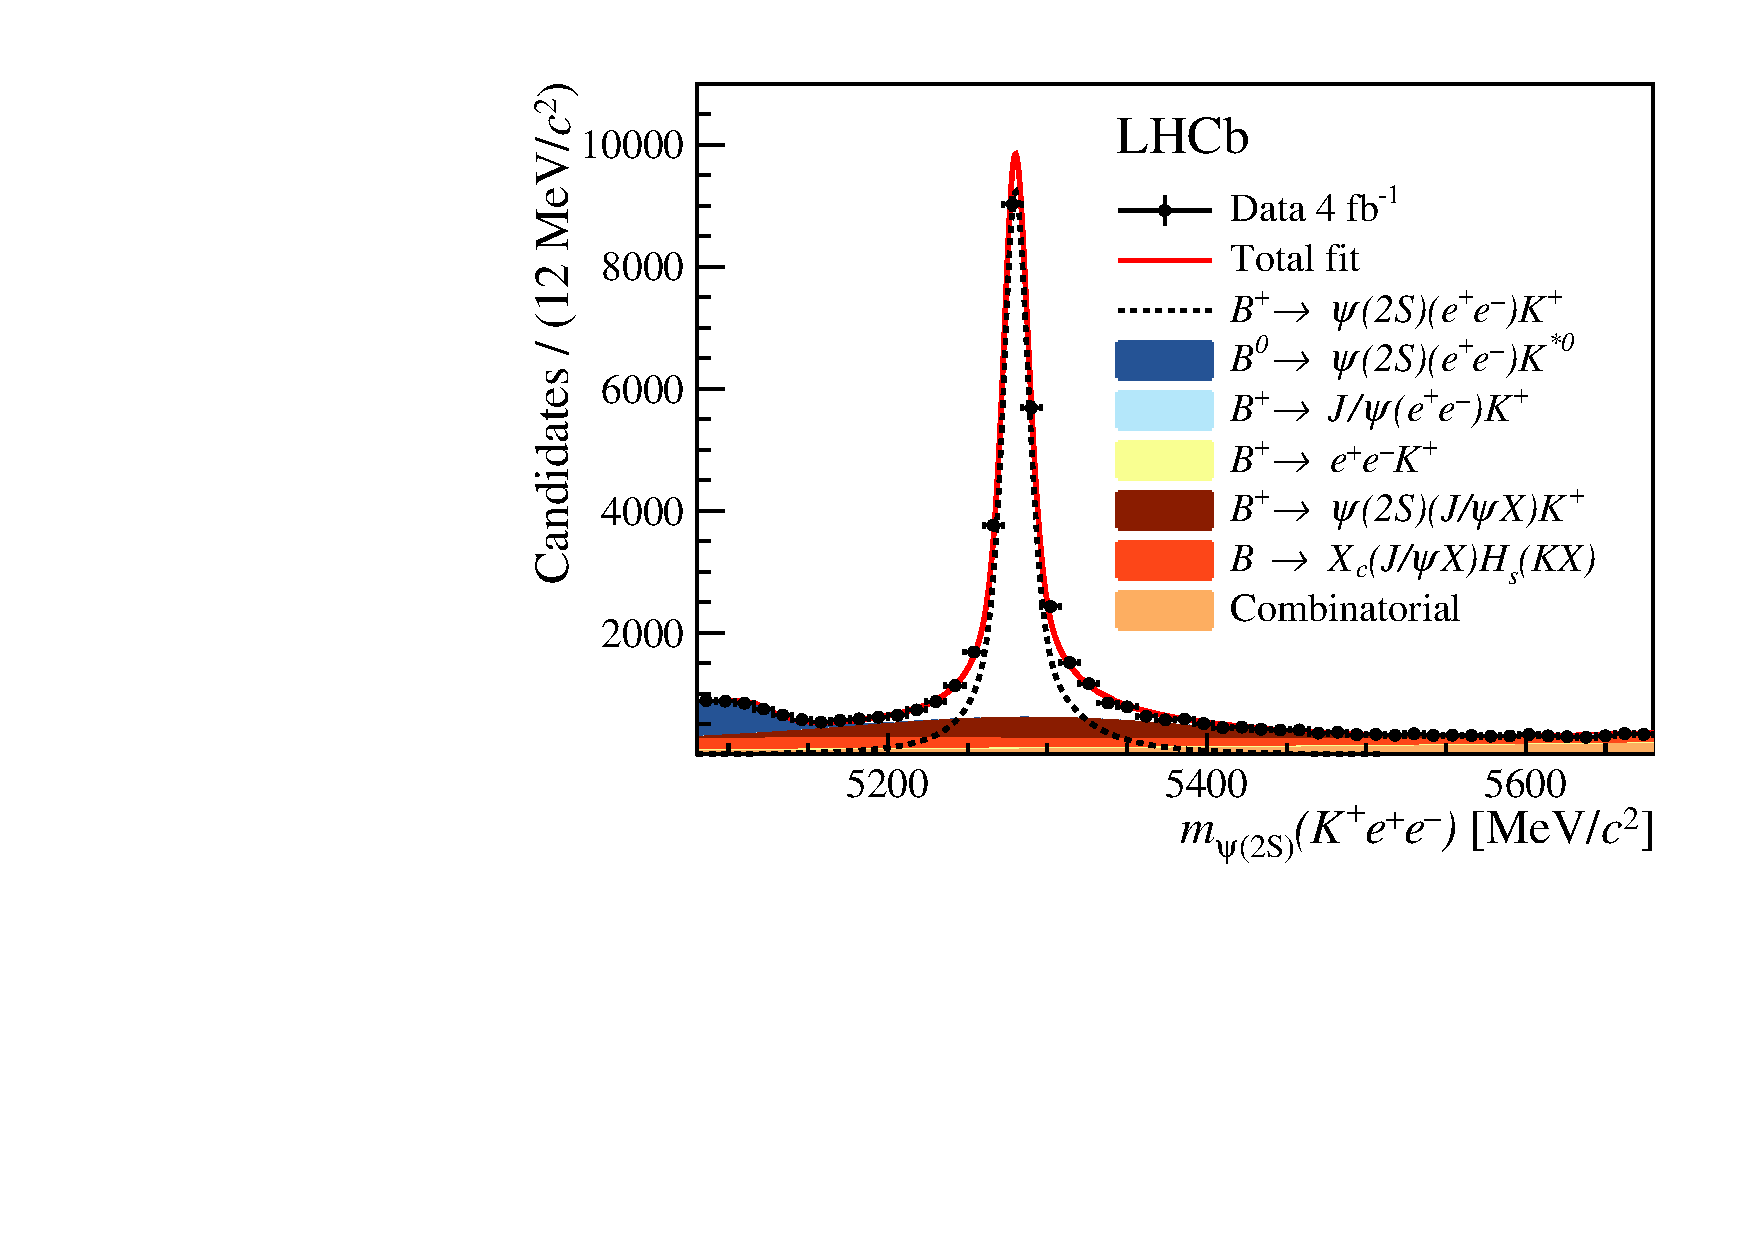
\includegraphics[width=0.45\textwidth]{figures/FigS2d.pdf}
    
    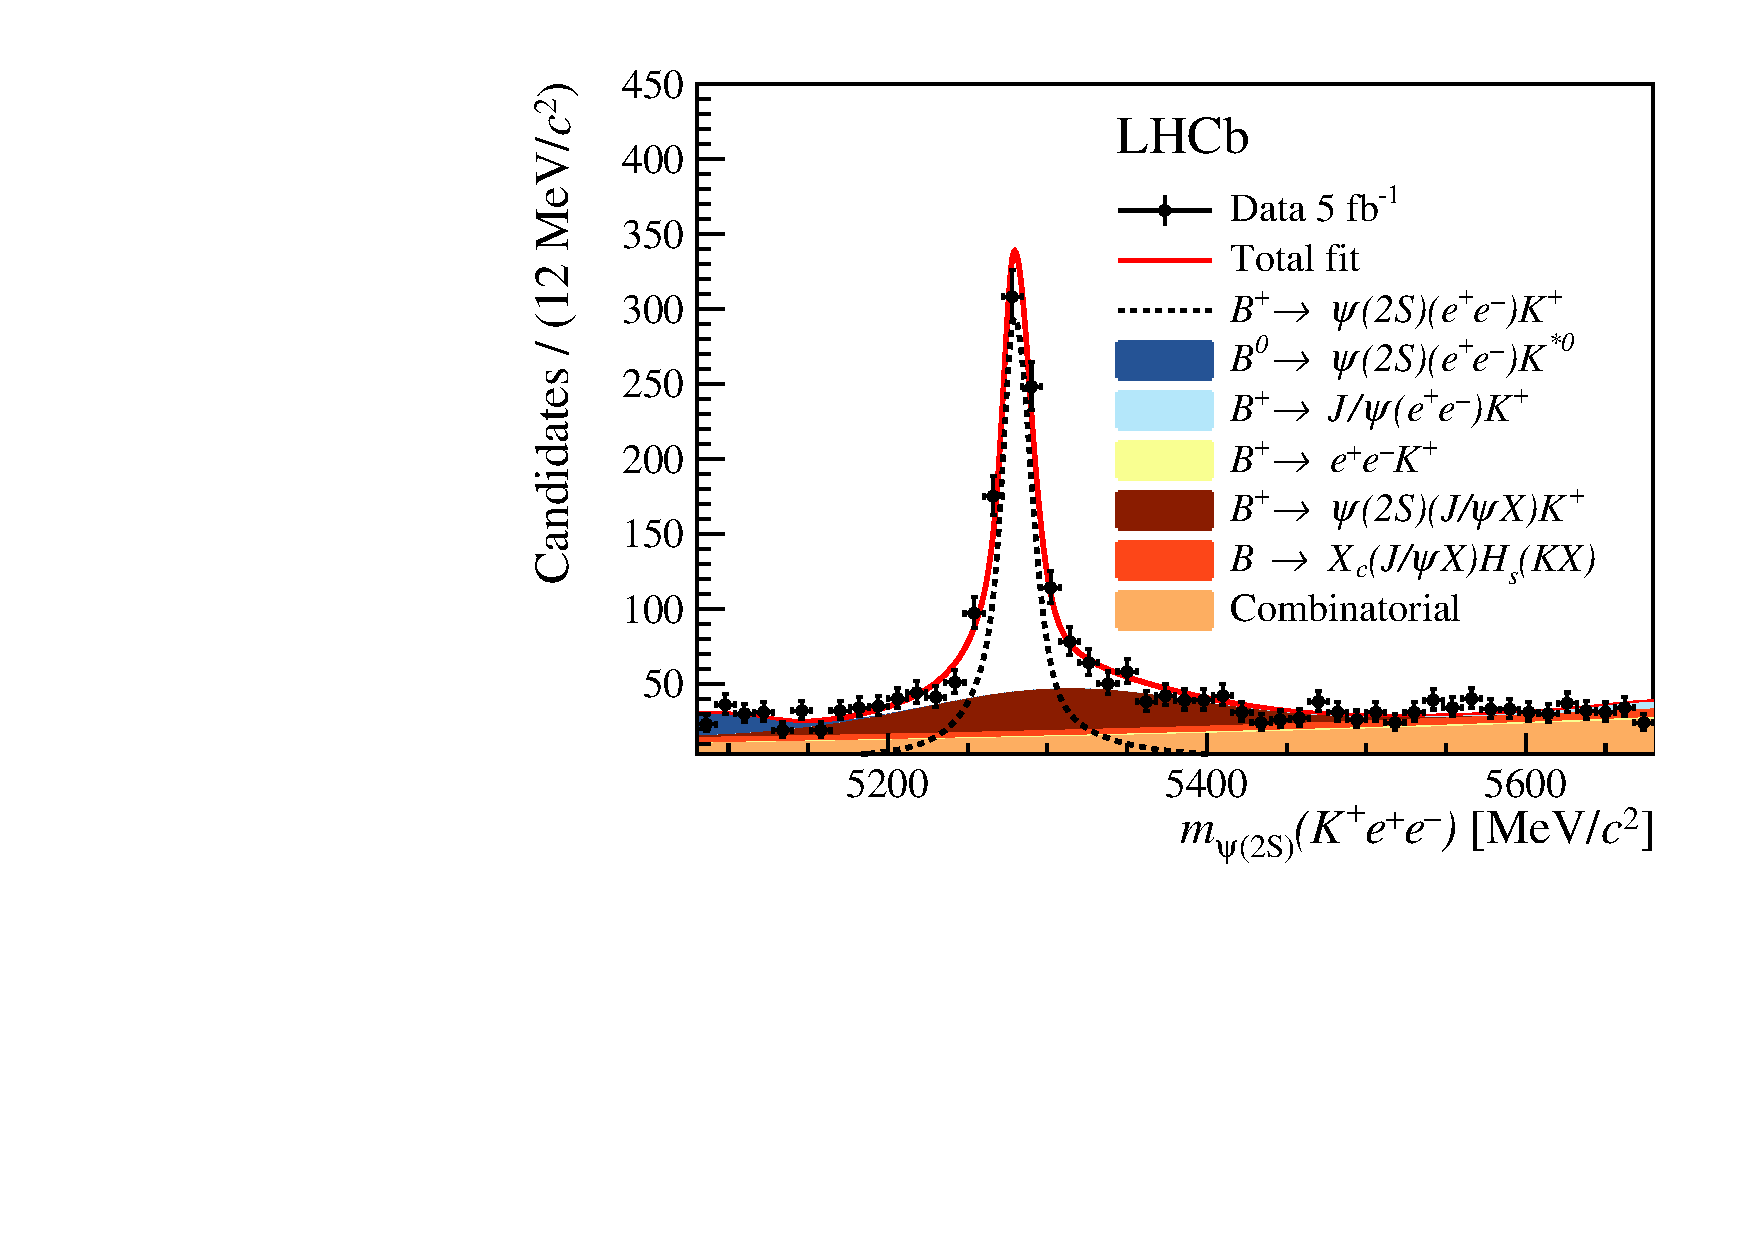
\includegraphics[width=0.45\textwidth]{figures/FigS2e.pdf}
    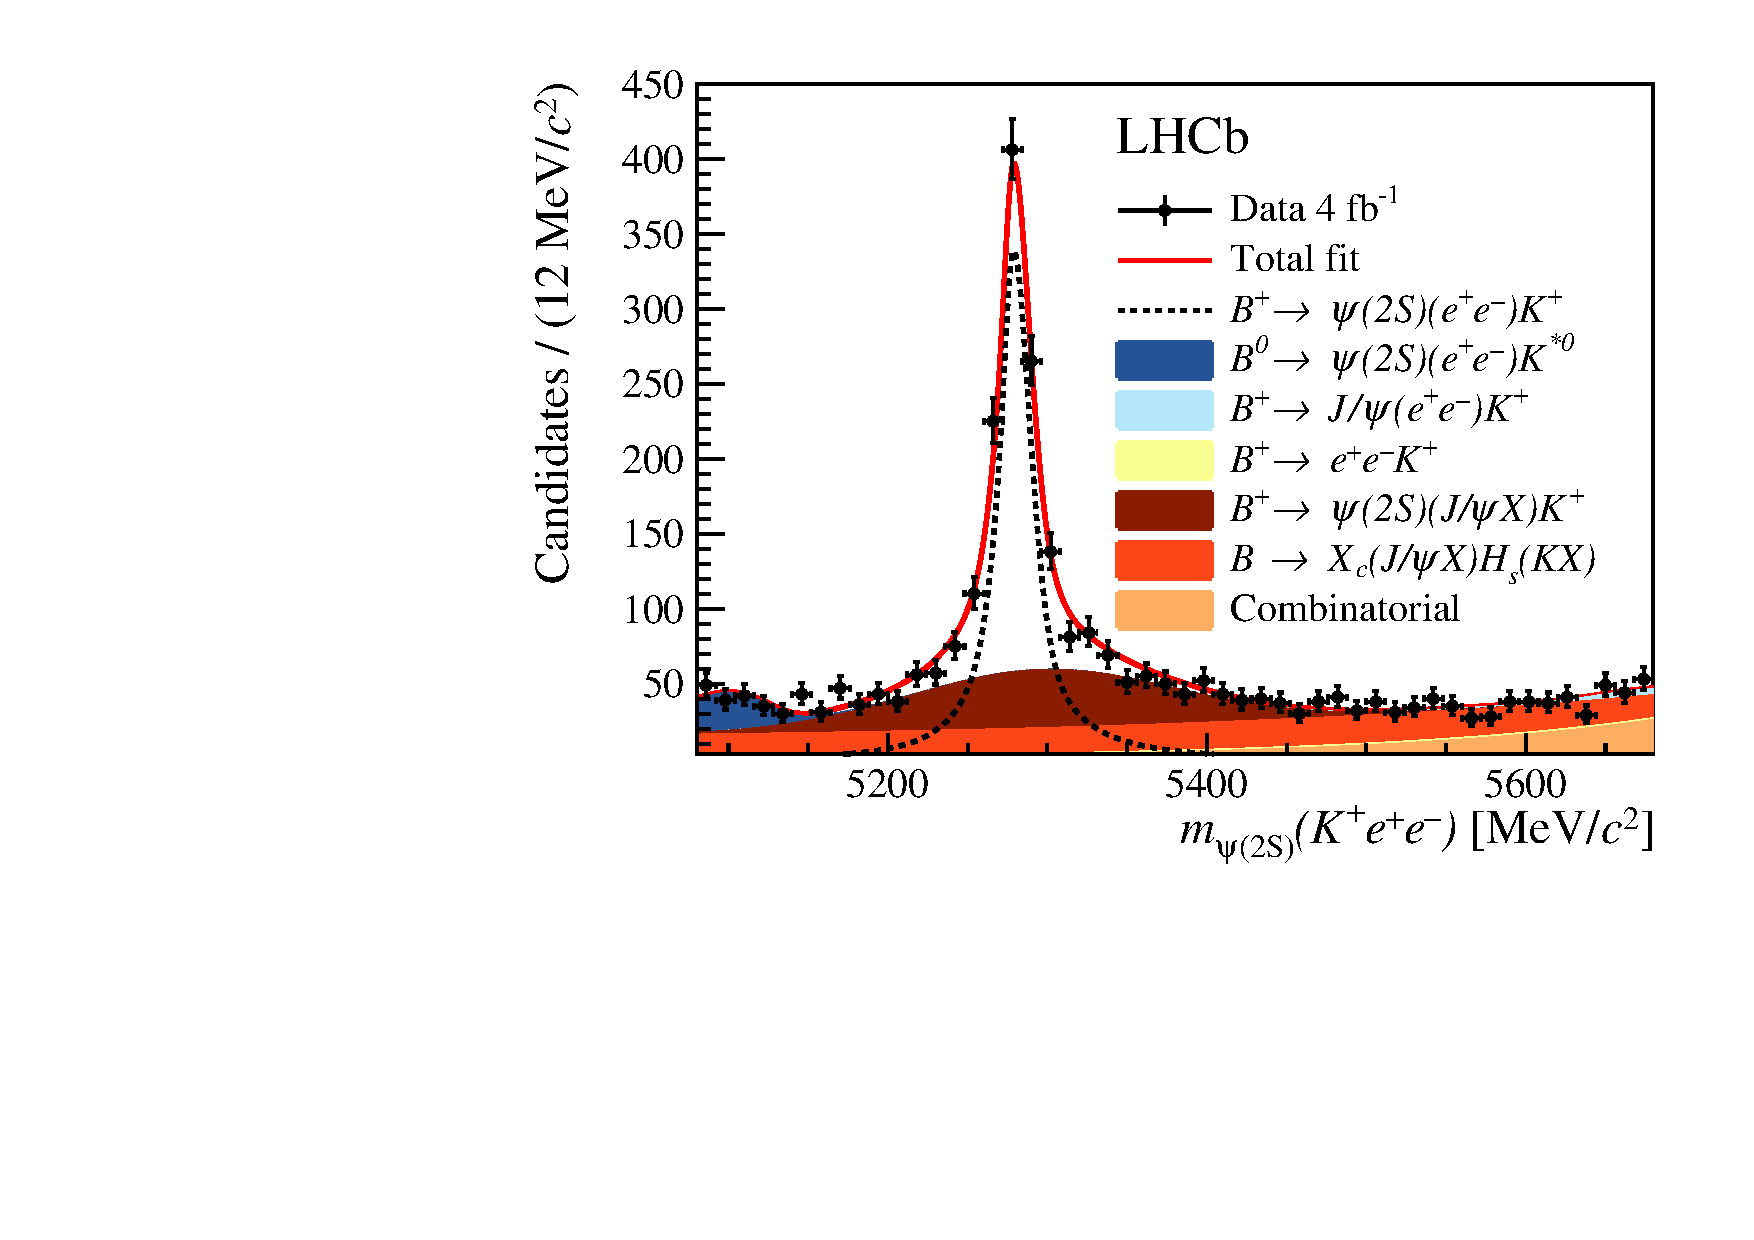
\includegraphics[width=0.45\textwidth]{figures/FigS2f.pdf}
    
    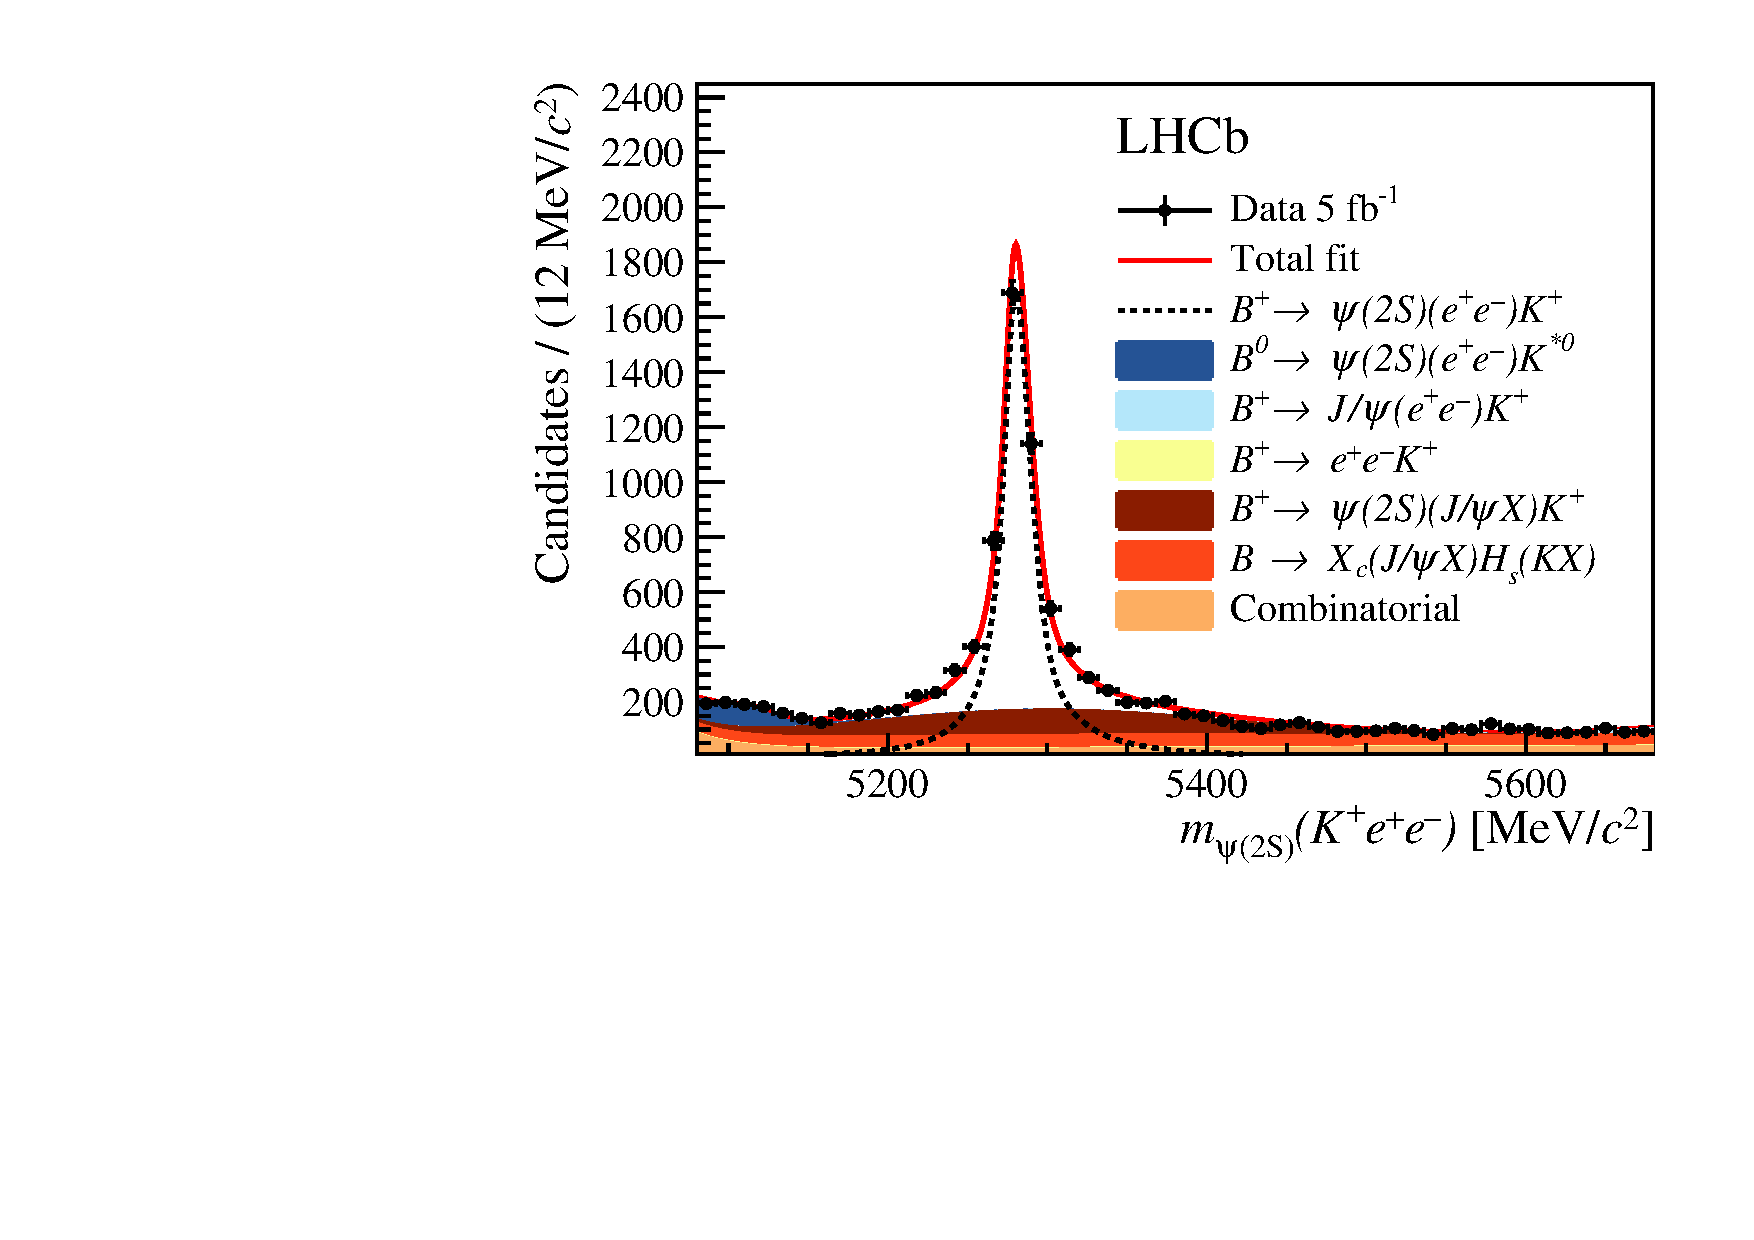
\includegraphics[width=0.45\textwidth]{figures/FigS2g.pdf}
    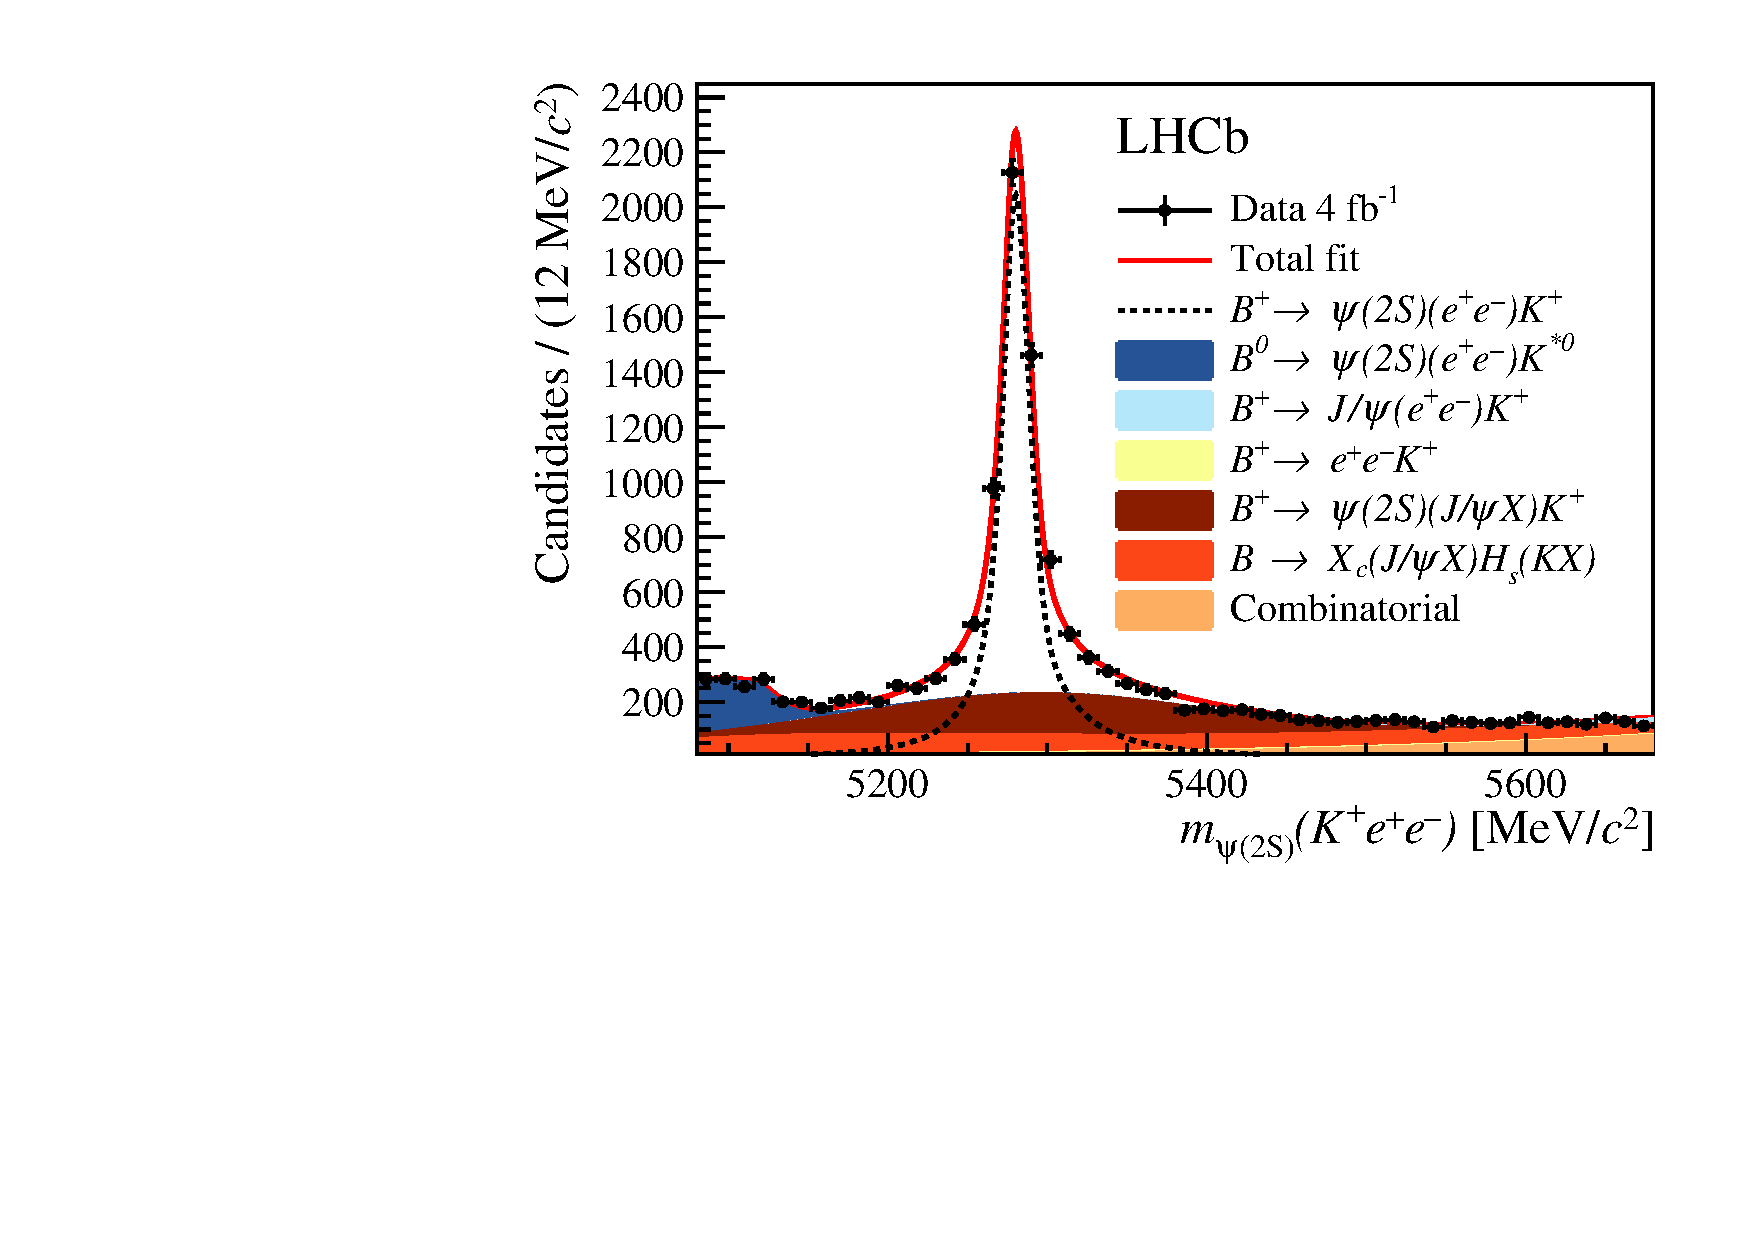
\includegraphics[width=0.45\textwidth]{figures/FigS2h.pdf}
    
    \caption{Candidate invariant mass distributions. Distribution of the invariant mass \mKllPsiSconst for \BuPsiK resonant candidates in the (left) sample previously analysed~\cite{LHCb-PAPER-2019-009} and (right) the new data sample. The top row shows the fit to the muon modes, the combinatorial component is included in the fit but is too small to be seen. The subsequent rows show the fits to the electron modes triggered by (second row) one of the electrons, (third row) the kaon and (last row) by other particles in the event. The fit projections are superimposed. 
%%    Some large pulls are observed but have a  negligible impact on %%the yields extracted.
}
    \label{fig:resPsi2Sfits_categories}
\end{figure}

\clearpage





\clearpage

\subsection*{Overview of {\boldmath \RK} measurements}

An overview of available measurements of \RK in different \qsq regions is given in Fig~\ref{fig:RKresultVSq2}. Previous LHCb measurements are also included for comparison in Fig~\ref{fig:RKresultVSq2Old} and Fig~\ref{fig:RKresultOld}.

\begin{figure}[!h]
    \centering
    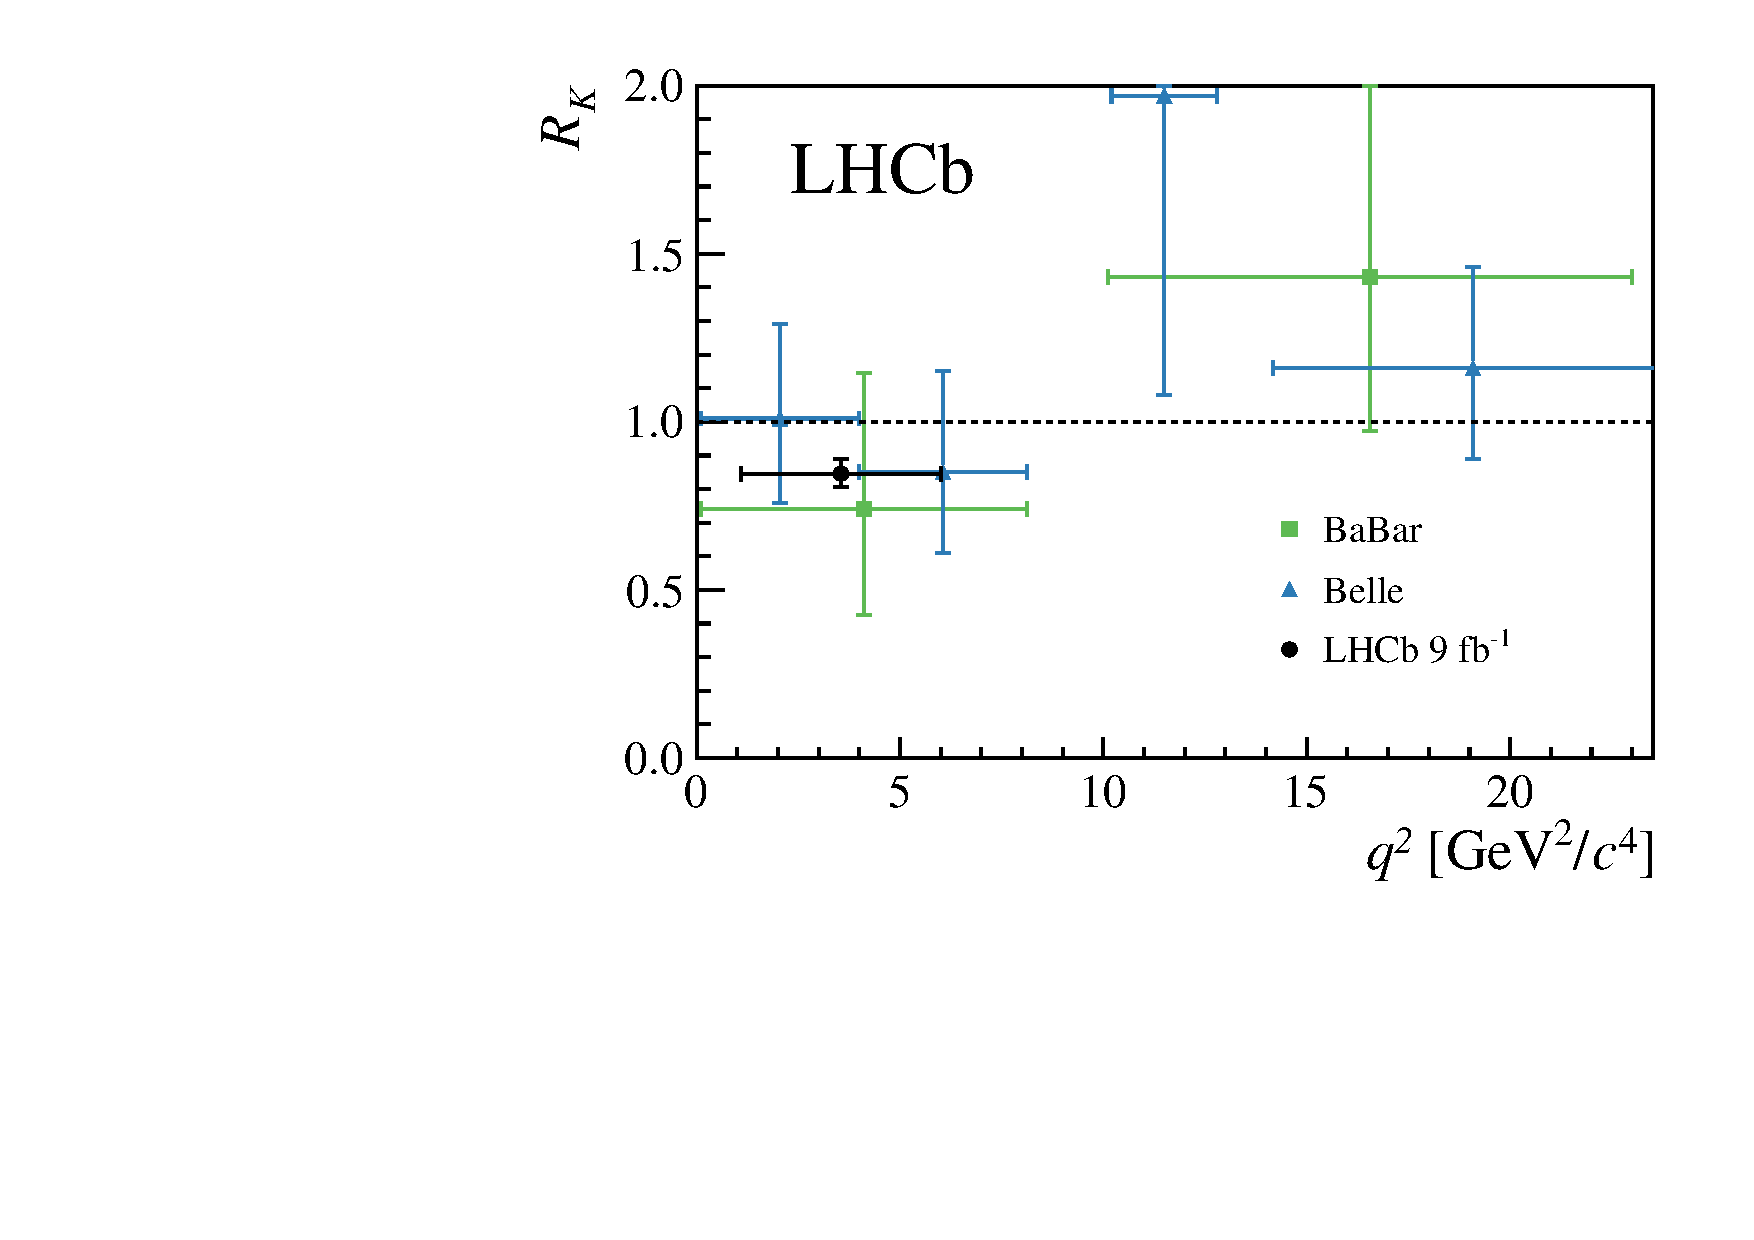
\includegraphics[width=0.7\textwidth]{figures/FigS3.pdf}
    \caption{Comparison between \RK measurements. 
    The measurements by the BaBar~\cite{RKbabar} and Belle~\cite{RKbelle} collaborations combine \BuKll and \BdKSll decays.}
    \label{fig:RKresultVSq2}
\end{figure}

\begin{figure}[!h]
    \centering
    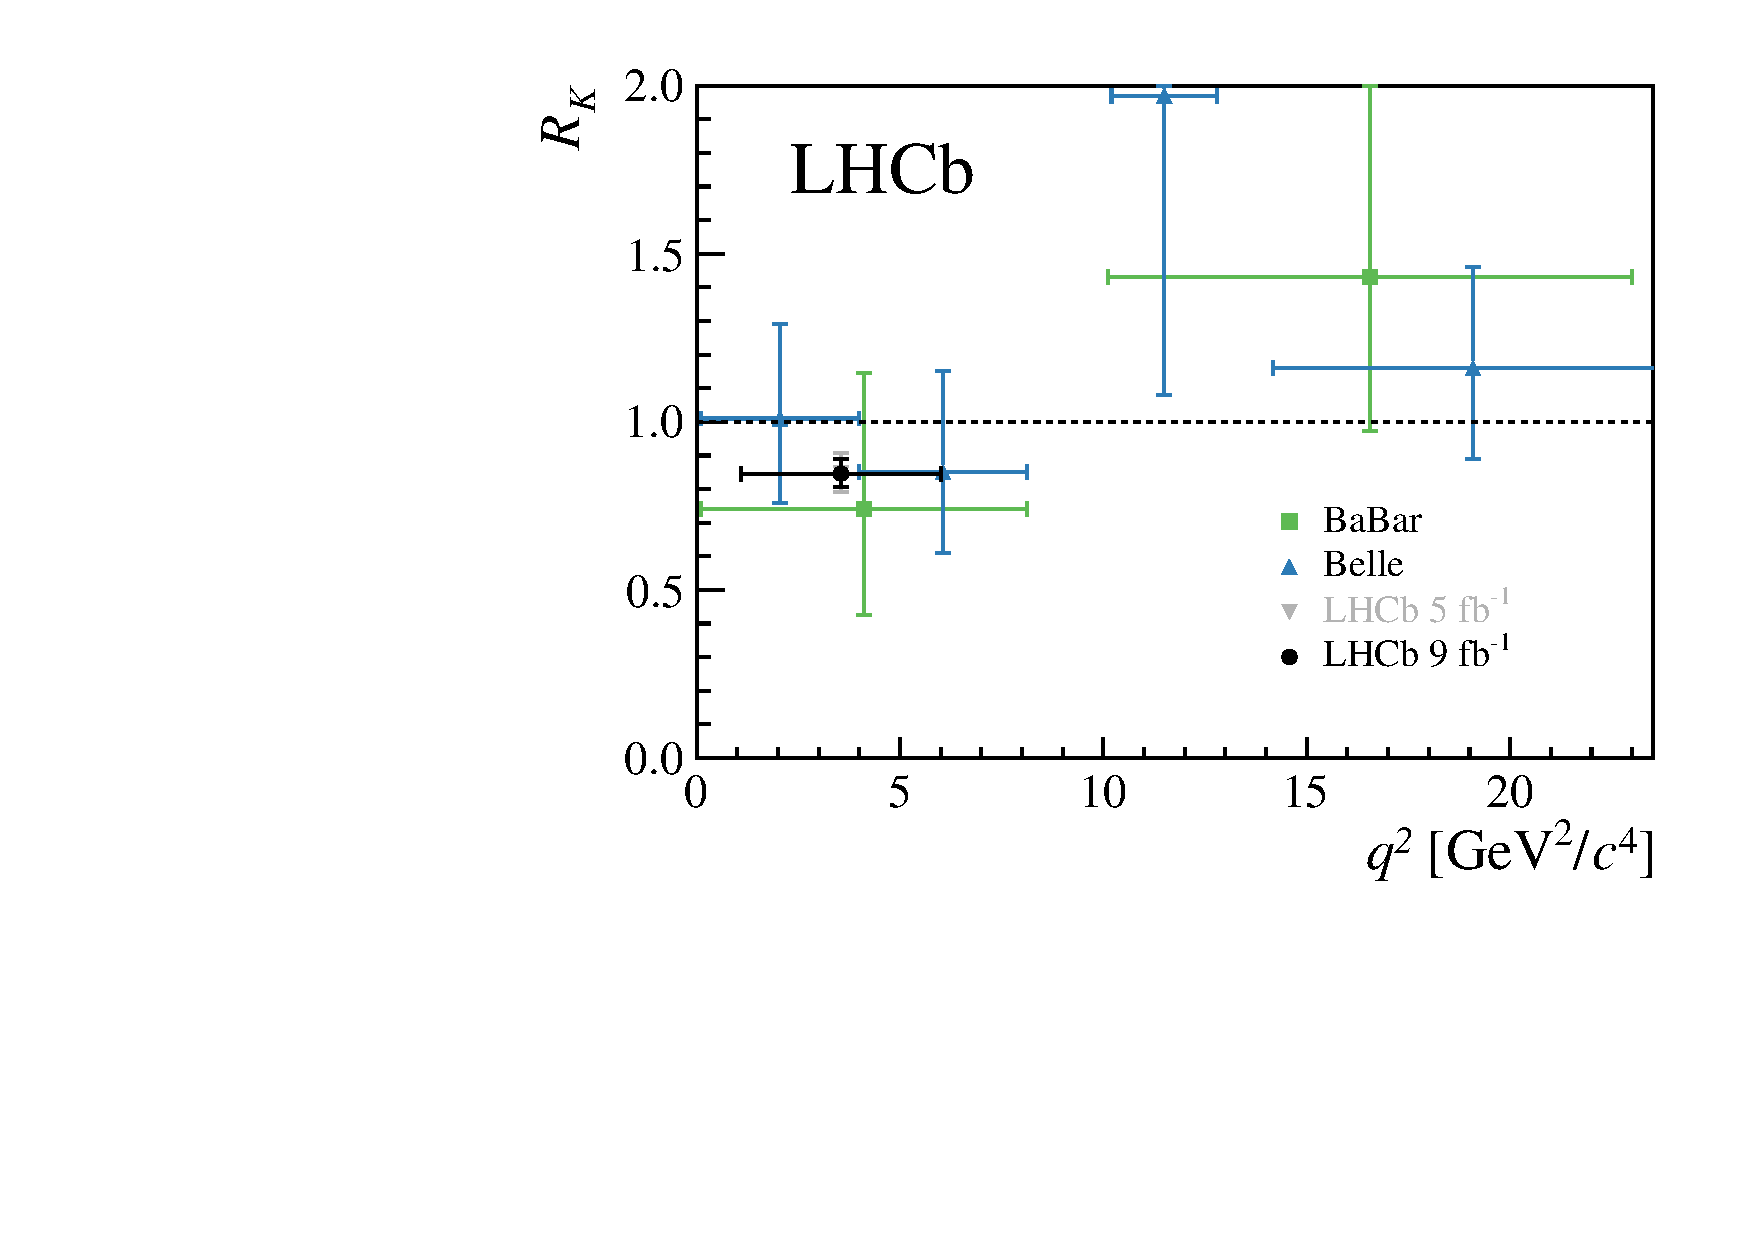
\includegraphics[width=0.7\textwidth]{figures/FigS4.pdf}
    \caption{Comparison between \RK measurements. 
    The measurements by the BaBar~\cite{RKbabar} and Belle~\cite{RKbelle} collaborations combine \BuKll and \BdKSll decays. The previous LHCb measurement~\cite{LHCb-PAPER-2019-009}, superseded by the present result, is also shown.
    \label{fig:RKresultVSq2Old}}
\end{figure}

\begin{figure}[!h]
    \centering
    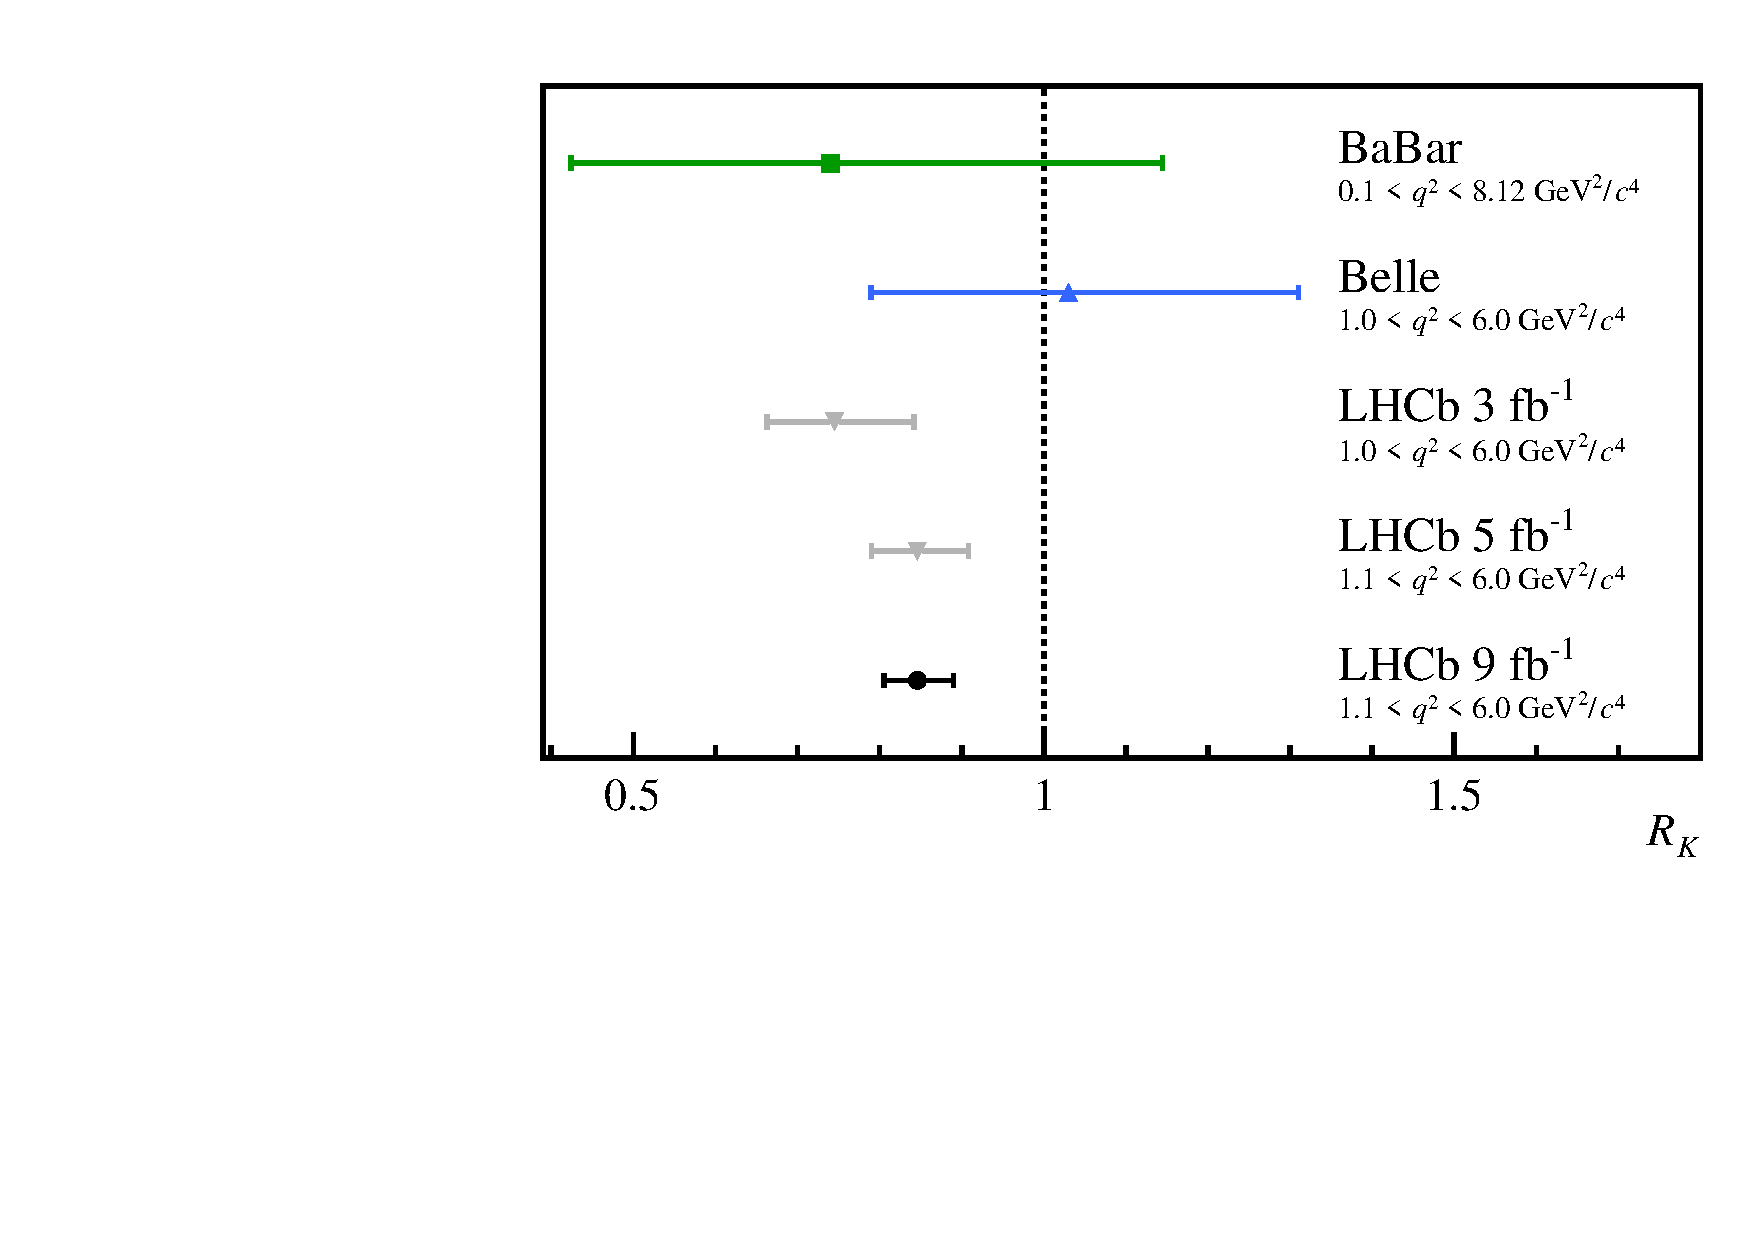
\includegraphics[width=0.7\textwidth]{figures/FigS5.pdf}
    \caption{Comparison between \RK measurements. 
    The measurements by the BaBar~\cite{RKbabar} and Belle~\cite{RKbelle} collaborations combine \BuKll and \BdKSll decays. The previous LHCb measurements~\cite{LHCb-PAPER-2019-009} and~\cite{LHCb-PAPER-2014-024}, superseded by the present result, are also shown.
    \label{fig:RKresultOld}}
\end{figure}